\addchap{Annex}

\begin{appendix}

\section*{Results}
\subsection*{Input Modality}
\subsubsection*{2x2 grid}
For the comparison between input modalities, we find that for the 2x2 grid, all mean accuracies across devices were higher for index finger tap data compared to classifiers trained with the thumb tap data. The iPhone 7 data yields the highest mean accuracy of 0.91 (+/- 0.07).

A Wilcoxon signed-rank test shows that the classification results for both input modalities differ significantly. The fold accuracies on thumb data were statistically lower than the fold accuracies on index finger data Z = 86.5, p < 0.05.

\begin{figure}[h!]
  \centering
  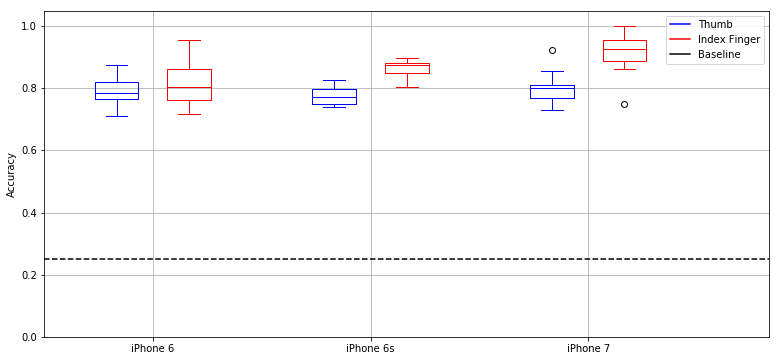
\includegraphics[width=1\textwidth]{results/index-vs-thumb-2x2.png}
  \caption{The figure shows the tap inference accuracies for the 2x2 grid of the 10-fold cross-validation.} \label{fig:participation}
\end{figure}

\begin{table}[h!]
  \centering
\begin{tabular}{|l|l|c|c|c|c|c|}
  \cline{3-7}
  \multicolumn{2}{c}{} & \multicolumn{4}{|c|}{\textbf{Accuracy}} & \textbf{Kappa} \\
  \hline
  \textbf{Device} & \textbf{Input Modality} & mean &   min &   max  & std &  mean \\
  \hline
	iPhone 6 & Index &      0.80 &     0.70 &     0.90 &     0.06 &        0.74 \\
	& Thumb &      0.80 &     0.74 &     0.85 &     0.03 &        0.73 \\
	\hline
iPhone 7 & Index &      0.91 &     0.78 &     1.00 &     0.06 &        0.88 \\
	& Thumb &      0.80 &     0.64 &     0.93 &     0.08 &        0.74 \\
	\hline
iPhone 6s & Index &      0.85 &     0.77 &     0.92 &     0.04 &        0.80 \\
	& Thumb &      0.78 &     0.71 &     0.85 &     0.04 &        0.70 \\
  \hline
\end{tabular}
  \caption{Classification results for the 2x2 tapping grid.}
\end{table}

\subsubsection*{4x3 grid}
For the 4x3, all mean accuracies across devices were higher for index finger tap data compared to classifiers trained with the thumb tap data. The greatest difference in inference accuracies are to found on the iPhone 7 where 0.72 (+/- 0.06) for index finger records and 0.53 (+/- 0.04) for thumb taps.

A Wilcoxon signed-rank test shows that the classification results for both input modalities differ significantly. The fold accuracies on thumb data were statistically lower than the fold accuracies on index finger data Z = 79.0, p < 0.05.


\begin{figure}[h!]
  \centering
  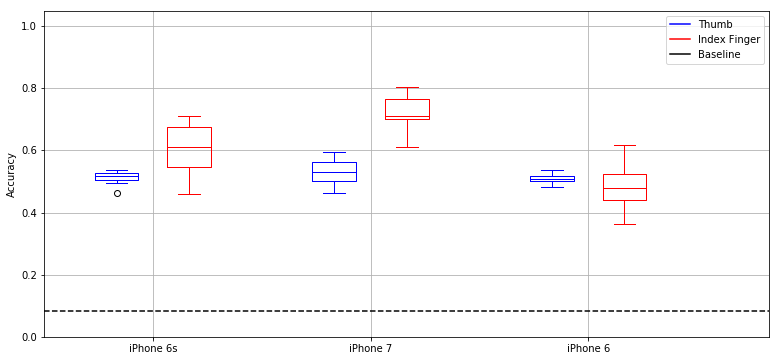
\includegraphics[width=1\textwidth]{results/index-vs-thumb-4x3.png}
  \caption{The figure shows the tap inference accuracies for the 4x3 grid of the 10-fold cross-validation.} \label{fig:participation}
\end{figure}

\begin{table}[h!]
  \centering
\begin{tabular}{|l|l|c|c|c|c|c|}
  \cline{3-7}
  \multicolumn{2}{c}{} & \multicolumn{4}{|c|}{\textbf{Accuracy}} & \textbf{Kappa} \\
  \hline
  \textbf{Device} & \textbf{Input Modality} & mean &   min &   max  & std &  mean \\
  \hline
	iPhone 6 & Index &      0.49 &     0.36 &     0.62 &     0.07 &        0.44 \\
	& Thumb &      0.51 &     0.48 &     0.54 &     0.02 &        0.47 \\
	\hline
iPhone 7 & Index &      0.72 &     0.61 &     0.80 &     0.06 &        0.69 \\
	& Thumb &      0.53 &     0.46 &     0.59 &     0.04 &        0.49 \\
	\hline
iPhone 6s & Index &      0.60 &     0.46 &     0.71 &     0.09 &        0.57 \\
	& Thumb &      0.51 &     0.46 &     0.54 &     0.02 &        0.47 \\
  \hline
\end{tabular}
  \caption{Classification results for the 4x3 tapping grid.}
\end{table}



\end{appendix}

\endinput
